%***************************************************************************************************************************

\chapter{Contraste de hipótesis}
El contraste de hipótesis, o lo que se conoce como tests estadísticos, se engloba en el ámbito de la
Inferencia Estadística, que es la parte de la estadística que estudia cómo sacar conclusiones generales
(sujetas a un determinado grado de fiabilidad o significancia) para toda la población a partir del
estudio de una muestra. En nuestro caso, se tratará de sacar conclusiones de los resultados obtenidos por
diferentes algoritmos (muestra) para determinar, por ejemplo, si los algoritmos tienen un rendimiento
significativamente diferente y por lo tanto no se pueden considerar iguales (población).

El \textbf{contraste de hipótesis} es uno de los problemas más comunes dentro de la inferencia
estadística. En él se contrasta una hipótesis estadística. Por ejemplo:\\\\
\textit{Un ingeniero de software afirma que la media de los resultados obtenidos por un algoritmo
de aprendizaje automático es 10. ¿Se podría desmentir la afirmación del ingeniero?}\\\\
El planteamiento del contraste sería el siguiente  ($\mu$ indica media poblacional):
\begin{center}
$ \mu = 10 $

$ \mu \neq 10 $
\end{center}

Para tomar una decisión (desmentir o no la afirmación), hay que basarse en los datos de una muestra, para
comprobar si en efecto la media de los resultados es 10 (media muestral). Para ello, podría establecer una
regla de decisión sobre la cual se basaría nuestra decisión final. Por ejemplo: si la media obtenida está
próxima a la afirmada por el ingeniero (10), entonces se podría afirmar que dice la verdad. Si por el
contrario la muestra nos proporciona una media muy distinta a 10, entonces se puede afirmar que la evidencia
desmiente la afirmación del ingeniero sobre el algoritmo en cuestión. Esto supone un problema y es el hecho
de cuándo considerar que la media es lo suficientemente distinta como para determinar que la afirmación del
ingeniero es errónea. Por ejemplo si la media de la muestra es 8.5, ¿se podría desmentir la afirmación
inicial? El contraste de hipótesis nos proporciona una forma de establecer este criterio y poder rechazar o
aceptar la afirmación inicial.

%***************************************************************************************************************************

\section{Hipótesis nula y alternativa}
En todo contraste de hipótesis siempre se dan dos posibilidades o hipótesis, las cuales se representan con
los siguientes símbolos:
\begin{center}
$H_0:$ Hipótesis nula

$H_1:$ Hipótesis alternativa
\end{center}
\begin{itemize}
\item $H_0$: Es la hipótesis que se supone cierta de partida, es decir, es la hipótesis que establece que lo que
indica la muestra es solamente debido a la variación aleatoria entre la muestra y la población.
\item $H_1$: Es la hipótesis alternativa y es la que reemplazará a la hipótesis nula si ésta es rechazada. $H_1$
establece que lo que indica la muestra es verdadero, ya que representa a toda la población.
\end{itemize}
A modo de ejemplo, supongamos que unos programadores están trabajando en la optimización de un algoritmo
de aprendizaje. El objetivo es mejorar el algoritmo de forma que los resultados que proporcione sean menores
de 100. Se toma una muestra de los resultados obtenidos por el nuevo algoritmo optimizado y se observa que la
media de la muestra es de 92. Si no hubiera incertidumbre en la media muestral, entonces se podría concluir
que la modificación reduciría los resultados a 92. Sin embargo, siempre existe incertidumbre en la media
muestral. La media poblacional en realidad será poco mayor o menor a 92.

Los programadores están preocupados de que el nuevo algoritmo en realidad no mejore al anterior, es decir, que
la media poblacional pudiera ser mayor o igual a 100. Quieren saber si esta preocupación está justificada. Se ha
observado una muestra con media de 92 y existen dos posibles interpretaciones o, como se ha mencionado más arriba
dos tipos de hipótesis que serán contrastadas más adelante mediante un determinado test estadístico:
\begin{enumerate}
\item La media poblacional es mayor o igual a 100 (la media muestral es, por tanto, menor debido sólo a la
variación aleatoria de la media poblacional). El nuevo algoritmo no mejorará al anterior.
\item La media poblacional es menor que 100, y la media muestral lo refleja. El nuevo algoritmo sí mejorará
al anterior.
\end{enumerate}
La primera interpretación sería la hipótesis nula o $H_0$. La segunda, la hipótesis alternativa o $H_1$, como bien
se comentó más arriba.

En este caso, los programadores están preocupados de que la hipótesis nula sea cierta. Un test estadístico o
prueba de hipótesis hallará una medida cuantitativa de la factibilidad de la hipótesis nula (denominado
estadístico de contraste, que para este ejemplo viene dado por la media obtenida en la muestra) y se podrá
decir a los programadores (después de que el test tome la decisión) si su preocupación está o no justificada.
Por tanto, a modo de resumen este ejemplo nos proporciona dos hipótesis:
$$H_0: \mu \geq 100 \mbox{ vs. } H_1: \mu < 100$$

La realización de un contraste de hipótesis no consiste en decidir cuál de las dos hipótesis ($H_0$, $H_1$) es más
creíble, sino en decidir si la muestra proporciona o no suficiente evidencia para descartar $H_0$. Para realizar la
prueba de hipótesis o test estadístico se pone la hipótesis nula en juicio, es decir se empieza suponiendo que $H_0$
es verdadera. Se podría poner como analogía el supuesto de \textit{``En un juicio, el acusado siempre es inocente
hasta que se demuestre lo contrario."} Esto es:
\begin{center}
$H_0:$ El acusado es inocente

$H_1:$ El acusado es culpable
\end{center}
y, mientras no se tenga suficiente evidencia para aceptar $H_1$, hay que creer que lo que dice $H_0$ es cierto. La
muestra aleatoria proporcionará la evidencia. Si el juicio (test o prueba de hipótesis) determina que el acusado
es inocente, sólo se puede decir que no se tiene suficiente evidencia para asegurar que el acusado es culpable,
mientras que si aceptamos la hipótesis alternativa, se estará bastante seguro de que el acusado sí es culpable.

%***************************************************************************************************************************

\section{Estadístico de contraste}
Los tests estadísticos o pruebas de hipótesis, calculan internamente una medida cuantitativa que proporciona la
factibilidad de la hipótesis nula. Esta medición se extrae de la muestra proporcionada. Por ejemplo, si queremos
contrastar la hipótesis de que la media poblacional es 5, un estadístico a calcular puede ser la media de una
muestra. En este caso, la muestra viene determinada por los resultados obtenidos por los algoritmos y cada uno de
los tests tiene una forma particular de hallar este estadístico mediante una fórmula que lo caracteriza. Estos
estadísticos siguen una determinada distribución de probabilidad. Por ejemplo en esta plataforma web, los tests
implementados harán uso de estadísticos que siguen distribuciones como:
\begin{itemize}
\item Distribución normal (p. ej. test de Wilcoxon).
\item Distribución chi cuadrado $\chi^2$ (p. ej. test de Friedman).
\item Distribución f de Fisher-Snedecor (p. ej. test de Iman-Davenport).
\item Distribución t de Student (p. ej. t-test).
\end{itemize}
La figura \ref{fig:pdf}, nos muestra el aspecto que presentan las distintas distribuciones de probabilidad. Las
distribuciones dependen de ciertos parámetros para determinar su forma ($\mu$, $\sigma^2$...): 
\begin{figure}[h]
\centering
\subfigure[Distribución normal con media $\mu$ y varianza $\sigma^2$.]{
\label{fig:pdfa}
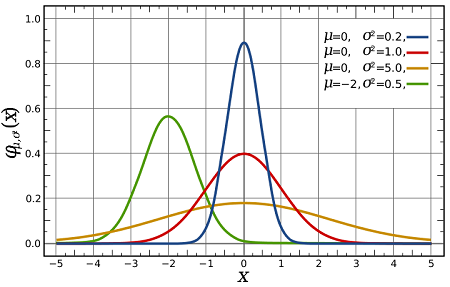
\includegraphics[width=5cm,height=3cm]{figuras/pdf_normal.png} }
\subfigure[Distribución chi cuadrado con $K$ grados de libertad.]{
\label{fig:pdfb}
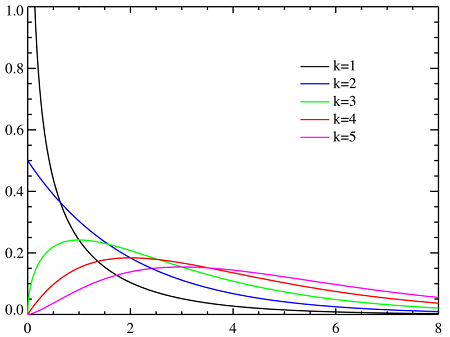
\includegraphics[width=5cm,height=3cm]{figuras/pdf_chi_cuadrado.png} }
\end{figure}
\begin{figure}[h]
\centering
\subfigure[Distribución f con $d1$ y $d2$ grados de libertad.]{
\label{fig:pdfc}
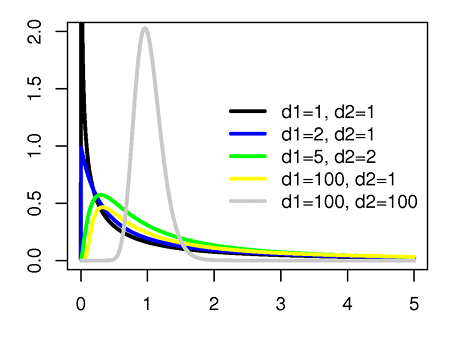
\includegraphics[width=5cm,height=3cm]{figuras/pdf_f.png} }
\subfigure[Distribución t con $K$ grados de libertad.]{
\label{fig:pdfd}
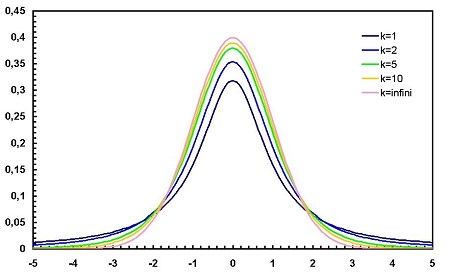
\includegraphics[width=5cm,height=3cm]{figuras/pdf_t_student.jpg} }
\caption{Funciones de distribución de probabilidad.}
\label{fig:pdf}
\end{figure}
\newline
Como podemos ver en la figura \ref{fig:pdf}, la distribución normal presenta $\mu$ y $\sigma^2$ como parámetros.
Éstos indican media y varianza respectivamente. La varianza, es una medida de dispersión que indica cómo se
distribuye la población. Por ejemplo: en una distribución normal de media 0 y varianza 1, que es la línea roja
en la figura \ref{fig:pdfa}, aproximadamente el $68\%$ de la población se encuentra en el intervalo $[-1,1]$,
ya que el área bajo la curva es de 0.68. Por tanto, la probabilidad de que un individuo de la población se
encuentre en ese intervalo es del 68\%. Si un estadístico sigue una distribución normal con media $\mu$ y
varianza $\sigma^2$, se expresa como:
\[ \mbox{Estadístico} \sim N(\mu,\sigma^2) \]
En las distribuciones chi cuadrado y t de Student se habla del parámetro $K$ o grados de libertad ($d1$ y $d2$  en
la distribución f de Fisher-Snedecor). La media y la varianza de estas tres distribuciones vendrán determinadas por
el parámetro $K$. Cuando se habla de grados de libertad se está refiriendo al número de valores que se pueden elegir
libremente en una muestra. Por ejemplo: una muestra con dos datos y media 5 si el primer dato toma el valor 4 entonces
necesariamente el segundo dato debe de ser 6 (para lograr la media de 5). En este caso,
se tienen:
\begin{center}
$N - 1$ grados de libertad, donde $N$ es el tamaño de la muestra.
\end{center}
Se hallan con la fórmula $N-R$, donde $N$ es el número de individuos en la muestra cuyo valor puede ser elegido de
forma libre y $R$ es el número de sujetos cuyo valor dependerá del valor que tengan los individuos de la muestra que
son libres. También se puede representar por $K-R$, donde $K$ es el número de grupos (cuando intervienen grupos y
no sujetos individuales).

En nuestro caso, $N$ viene determinado por el número de resultados obtenidos por los algoritmos (número de filas
de la matriz de la muestra de datos) y $K$ por el número de algoritmos o variables relacionadas que tiene la muestra
de datos con la que se están aplicando los tests (número de columnas de la matriz). Cada test que use el parámetro
de grados de libertad lo calcula de acuerdo a su fórmula característica para el estadístico. 

Todas las distribuciones de la figura \ref{fig:pdf} son continuas, pues se puede tomar cualquier valor dentro de un
intervalo, a diferencia de las distribuciones discretas. Por otra parte, en la distribución t de Student a medida que
aumentan los grados de libertad se tiende más a una distribución normal estandarizada (de $\mu = 0$ y $\sigma^2 = 1$).

Las distribuciones de probabilidad que puedan seguir un estadístico nos dan un valor diferente de probabilidad para
cada valor diferente del estadístico. Este valor de probabilidad indica cómo de probable que es obtener ese valor del
estadístico siendo la hipótesis nula cierta. Por ejemplo, si es cierta la hipótesis nula de que la media de una población
es 5, es más probable que obtengamos una media de una muestra igual a 4.5 que a 3.

%***************************************************************************************************************************

\section{Decisiones y tipos de error}
Cuando se lleva a cabo un contraste de hipótesis sólo se pueden tomar dos decisiones. Los datos de la muestra,
que en este proyecto vendrá dada por los resultados obtenidos por los algoritmos, evidenciarán qué decisión se
debe tomar:
\begin{enumerate}
\item Aceptar la hipótesis nula ($H_0$) (Rechazar la hipótesis alternativa $H_1$)
\item Rechazar $H_0$ (Aceptar la hipótesis alternativa)
\end{enumerate}
Sin embargo, cuando se toma la decisión se pueden cometer dos tipos de error. La figura \ref{fig:decision}, nos
muestra las decisiones y los dos tipos de errores que se pueden cometer:
\begin{figure}[h]
\centering
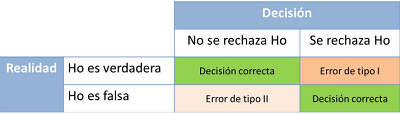
\includegraphics[width=7cm,height=2cm]{figuras/figura1.png}
\caption{Decisiones y tipos de error.}
\label{fig:decision}
\end{figure}
\newpage
La probabilidad de ``Error tipo I" se denota por $\alpha$ y se denomina nivel de significación:
\begin{center}
$P(\mbox{``Error tipo I}") = P(\mbox{Rechazar } H_0|H_0 \mbox{ es cierta}) =\alpha$
\end{center}
El nivel de significación consiste en la probabilidad de rechazar la hipótesis nula $H_0$ cuando verdaderamente
es cierta. Este valor $\alpha$ es un parámetro que debe seleccionar la persona que quiere realizar un test
estadístico en base a cómo de importante considere rechazar $H_0$ cuando es cierta. Normalmente es del 5\%, lo
que implicará que 5 de cada 100 veces se acepta la hipótesis alternativa cuando la cierta es la hipótesis nula.
Cuanto menor sea el nivel de significación, cada vez es más difícil rechazar la hipótesis nula. Es decir, si
queremos equivocarnos menos veces, necesitamos mucha más evidencia para justificar el rechazo. Si es grande es
más fácil aceptar la hipótesis alternativa cuando en realidad es falsa.
\\Por otra parte, la probabilidad de ``Error tipo II" se denota por $\beta$:
\begin{center}
$P(\mbox{``Error tipo II}") = P(\mbox{Aceptar } H_0|H_0 \mbox{ es falsa}) =\beta$
\end{center}
Este error $\beta$ consiste en la probabilidad de aceptar la hipótesis nula $H_0$ cuando verdaderamente es
falsa.
\\Por último, cabe destacar el concepto de ``Potencia".
\begin{center}
$P(\mbox{``Potencia}") = P(\mbox{Rechazar } H_0|H_0 \mbox{ es falsa}) =1-\beta.$
\end{center}
La potencia es la probabilidad de detectar que una hipótesis es falsa. Los tests estadísticos o pruebas de hipótesis
implementados en el presente proyecto se caracterizan por su potencia, siendo esta fija, y dejando como parámetro
libre el nivel de significación. Así, cuanto mayor es el nivel de potencia, mejor será el test, ya que se rechazarán
más hipótesis nulas cuando se deben rechazar (mayor habilidad en aceptar correctamente hipótesis alternativas).

En este proyecto se pondrá el énfasis en el nivel de significación, ya que es la hipótesis alternativa la que se
quiere probar y no se quiere aceptar si en realidad no es cierta, es decir, si aceptamos la hipótesis alternativa
queremos equivocarnos con un margen de error muy pequeño. Obviamente, lo ideal sería que tanto $\alpha$ como
$\beta$ fuesen nulos y que no se cometiese ningún error, o que ambos valores fuesen muy pequeños. Como no se pueden
disminuir ambos errores a la vez, se controla el ``Error tipo I".

%***************************************************************************************************************************

\section{Intervalos de confianza}
El nivel de significación fijado divide en dos regiones el conjunto de posibles valores del estadístico de
contraste: la región de aceptación y la región de rechazo o región crítica. Se denomina región de aceptación
a la región que conduce a la aceptación de $H_0$ y región de rechazo a la región que conduce al rechazo de $H_0$
en favor de $H_1$. Aquí surge el concepto de ``Cola", que indica la porción o porciones de una distribución
de probabilidad en la cual se rechaza la hipótesis nula.

La determinación de las regiones de aceptación o de rechazo depende de cómo se establezca la hipótesis
alternativa $H_1$. Por ejemplo, si hablamos de un contraste en el que se esté contrastando una determinada
media ($\mu_0$) se podría establecer como $H_1$ que la media en realidad sea menor, mayor o distinta a
($\mu_0$):\\\\
\begin{itemize}
\item Media menor (test unilateral con cola a la izquierda):
\end{itemize}
\begin{center}
$H_0: \mu = \mu_0$
\\$H_1: \mu < \mu_0$
\end{center}
\begin{itemize}
\item Media mayor (test unilateral con cola a la derecha):
\end{itemize}
\begin{center}
$H_0: \mu = \mu_0$
\\$H_1: \mu > \mu_0$
\end{center}
\begin{itemize}
\item Media distinta (test bilateral o de dos colas):
\end{itemize}
\begin{center}
$H_0: \mu = \mu_0$
\\$H_1: \mu \neq \mu_0$
\end{center}
En la figura \ref{fig:intervalos_normal}, podemos ver cómo quedarían establecidos los intervalos para el ejemplo:
\begin{figure}[h]
\centering
\subfigure[Test unilateral. Cola a la izquierda.]{
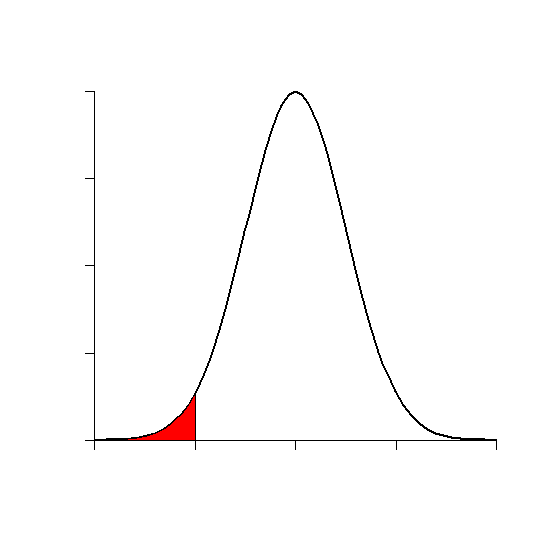
\includegraphics[width=5cm,height=3cm]{figuras/test_unilateral_izq.png} }
\subfigure[Test unilateral. Cola a la derecha.]{
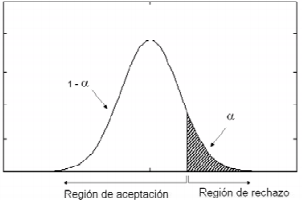
\includegraphics[width=5cm,height=3cm]{figuras/test_unilateral_der.png} }
\end{figure}
\begin{figure}[h]
\centering
\subfigure[Test bilateral o de dos colas.]{
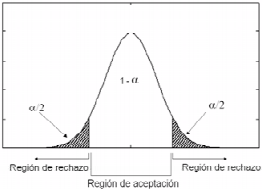
\includegraphics[width=5cm,height=3cm]{figuras/test_bilateral.png} }
\caption{Regiones de aceptación y rechazo.}
\label{fig:intervalos_normal}
\end{figure}

%***************************************************************************************************************************

\section{Decisión final y Concepto de p-valor}
Si el valor del estadístico cae en la región de aceptación, se acepta la hipótesis nula, ya que no existen
razones suficientes para rechazar $H_0$ con el nivel de significación dado. Por tanto, en este caso se diría
que el contraste es estadísticamente no significativo, es decir, no existe evidencia estadísticamente significativa
en favor de $H_1$.
\begin{figure}[h]
\centering
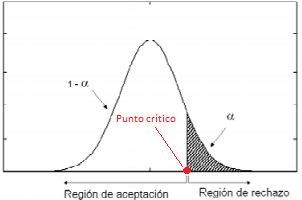
\includegraphics[width=5cm,height=3cm]{figuras/test_unilateral_critico.png}
\caption{Punto crítico.}
\label{fig:punto_critico}
\end{figure}
La figura \ref{fig:punto_critico} nos muestra el punto crítico: si el estadístico obtenido por el test o
prueba de hipótesis es 5 y el punto crítico es 4.5, se rechaza $H_0$ ya que el estadístico pertenece a la
región de rechazo.

La decisión de rechazar o aceptar la hipótesis nula, se puede determinar también mediante el p-valor,
que es el parámetro utilizado para realizar los tests estadísticos en este proyecto. El p-valor proporciona
un forma más eficiente de determinar si el contraste es o no estadísticamente significativo, ya que no sería
necesario recalcular regiones de aceptación y rechazo cada vez que el usuario de los tests cambia de nivel de
significación.

%***************************************************************************************************************************

\section{Etapas en la resolución de un contraste de hipótesis}
En un contraste de hipótesis siempre se siguen una serie de pasos definidos. Como se ha ido viendo a lo largo
del capítulo, los pasos para la realización de una prueba de hipótesis o test estadístico son las siguientes:
\begin{enumerate}
\item Especificación de la hipótesis nula $H_0$ y de la hipótesis alternativa $H_1$.
\item Suponer que $H_0$ es verdadera (el test sirve para que a partir de la muestra de datos podamos rechazar
$H_0$ en beneficio de $H_1$).
\item Calcular un estadístico de prueba o estadístico de contraste. Este estadístico se usa para evaluar la
fuerza de la evidencia en contra de $H_0$ (medir la discrepancia entre la hipótesis y la muestra).
\item Establecer un nivel de significación $\alpha$ en base a cómo de importante se considere rechazar $H_0$
cuando realmente es verdadera.
\item El nivel de significación fijado divide en dos regiones el conjunto de posibles valores del estadístico
de contraste: la región de aceptación y la región de rechazo o región crítica.
\item Si el valor del estadístico cae en la región de rechazo, se rechaza la hipótesis nula, ya que esto
evidencia que los datos obtenidos de la muestra no son compatibles con $H_0$. Por tanto, en este caso se diría
que el contraste es estadísticamente significativo, es decir, existe evidencia estadísticamente significativa en
favor de $H_1$.
\item Si el valor del estadístico cae en la región de aceptación, se acepta la hipótesis nula, ya que no existen
razones suficientes para rechazar $H_0$ con el nivel de significación dado. Por tanto, en este caso se diría
que el contraste es estadísticamente no significativo, es decir, no existe evidencia estadísticamente significativa
en favor de $H_1$.
\item La decisión de rechazar o aceptar la hipótesis nula, se puede determinar también mediante el p-valor,
que es el parámetro utilizado para realizar los tests estadísticos en este proyecto. El p-valor proporciona
un forma más eficiente de determinar si el contraste es o no estadísticamente significativo, ya que no sería
necesario recalcular regiones de aceptación y rechazo cada vez que el usuario de los tests cambia de nivel de
significación.
\end{enumerate}

%***************************************************************************************************************************

\section{Tests paramétricos y no paramétricos}
